\textit{Into this chapter, we discuss the fact that over the last years, the Web of Data has grown significantly. Various interfaces such as LOD Stats, LOD Laudromat, SPARQL endpoints provide access to the hundered of thousands of RDF datasets, representing billions of facts. These datasets are available in different formats such as raw data dumps and HDT files or directly accessible via SPARQL endpoints. Querying such large amount of distributed data is particularly challenging and many of these datasets cannot be directly queried using the SPARQL query language. In order to tackle these problems, we present WimuQ, an integrated query engine to execute SPARQL queries and retrieve results from large amount of heterogeneous RDF data sources. Presently, WimuQ is able to execute both federated and non-federated SPARQL queries over a total of 668,166 datasets from LOD Stats and LOD Laudromat as well as 559 active SPARQL endpoints. These data sources represent a total of 221.7 billion triples from more than 5 terabytes of information from datasets retrieved using the service ``Where is My URI'' (WIMU). Our evaluation on state-of-the-art real-data benchmarks shows that WimuQ retrieves more complete results for the benchmark queries. }	

\section{Introduction}
\label{sec:intro}
%\todo[inline]{Include again: Preliminaries, research questions, hypothesis, include a table comparing the approaches, more metrics etc...}

Currently, the LOD Laudromat along with LOD stats have more than 250 billion facts which are available on 668,166 datasets and 559 active SPARQL endpoints~\cite{valdestilhas2018my}. Querying such large amount of distributed data is particularly challenging in which Federated query processing is one of the key components for accessing this collection of information through these data sources. In general, there are two types of available approaches to execute federated SPARQL queries over distributed RDF data sources~ \cite{saleem2015fine}. (1) \texttt{Query federation over multiple SPARQL endpoints (QFME)} which collects distributed information from multiple SPARQL endpoints. Commonly, the list of SPARQL endpoints is provided as an input to the federation engine. The federation engine decomposes the original query into multiple sub-queries and execute them accordingly to a specific query execution plan. (2) \texttt{Link Traversal based SPARQL federation (LTSF)} which uses the URI lookups to collect information from distributed RDF data sources. Such approaches do not force the data providers to publish their data as SPARQL endpoints. Instead, the only requirement is that the RDF data sources must follow the Linked Data principles\footnote{\url{http://www.w3.org/DesignIssues/LinkedData.html}}~\cite{hartig2013overview}. 

%, which makes use of the endpoint URLs to federate sub-queries according to the generated query execution plan. 
%The sub-queries results are then integrated locally by the federation engine and sent back to the user. 
%The advantage of this category of approaches is that the query execution workload is distributed between SPARQL endpoints and the federation engine. Consequently, execution of queries can be carried out efficiently if the federation engine is able to intelligently distribute the query workload among SPARQL endpoints \cite{saleem2015fine}. 
%queries are answered based on original, up-to-date data with no synchronization of the copied data required~\cite{hartig2013overview}. 
%Moreover, the execution of queries can be carried out efficiently because the approach relies on SPARQL endpoints. 
%However, such approaches are unable to deal with the data provided by the whole of LOD Cloud because sometimes Linked Data is not exposed through SPARQL endpoints.
However, a particular shortcoming of the QFME approaches is that many of the RDF datasets in Linking Open Data (LOD) are not publicly available via SPARQL endpoints. Beek et al.~\cite{beek2014lod} has shown that around 90\% of the information published are available only as data dumps. On the other hand, the LTSF approaches are unable to perform lookups for non-dereferenceable URIs. Hence, they may retrieve empty or incomplete results for the latter type of approaches. Note that our previous work~\cite{valdestilhas2018my} shows that around 43\% of the URIs of more than 660K RDF datasets from LODStats~\cite{ermilov2016lodstats} and LODLaundromat~\cite{beek2014lod} are non-dereferenceable. 
%The set of data sources which can contribute results into the final query resultset is determined by using URI lookups during the query execution itself. 
%Query federation over Linked Data does not require the data providers to publish their data as SPARQL endpoints. 
%Instead, the only requirement is that the RDF data follows the Linked Data principles. 
%A downside of these approaches is that they are less time-efficient than the previous approaches due to the URI lookups they perform. 
%Starting by using an analogy. Suppose that you have a question, but you do not know to whom you will ask, nowadays, someone can just answer, just put your question on Google. Similarly, in case you do not know which dataset to execute a SPARQL query, you can use a Traversal SPARQL query engine.
%URI dereferencing is the process of looking up a URI on the Web in order to access the referenced resource  \cite{jacobs2004architecture}. 
%where Items of interest are called resources and are identified by URIs, in which Web agents may retrieve representations of resources by dereferencing URIs. 
%An RDF representation of a resource is retrieved by dereferencing the resource URI with an HTTP request asking for content type application/rdf+xml\cite{bizer2006d2r}. 
%For linked data, it is possible to dereference URIs during query processing to access remote data sources at runtime. 
%A number of approaches have looked at  such the Link-Traversal Based Query Execution (LTBQE) approaches. LTBQE has the advantage to provide up-to-date results and decentralized (i.e., client-side) execution. On the other hand, it must operate over incomplete dereferenceable knowledge available in remote data sources, thus affecting response times~\cite{umbrich2015link} and completeness for query answers.

%In order to tackle these problems, we present WimuQ which is an approach to execute SPARQL queries over large amount of heterogeneous RDF data sources. Additionally, our approach is able to identify automatically the datasets where these SPARQL queries can retrieve results thus improving the completeness.

%In what follows, we first describe an example of real-world scenario and then describe the unique challenge not addressed in previous work.
%Let us consider the given problem, a user or a system that usually executes queries on a dataset or a collection of datasets which suddenly stop to work , e.g., the SPARQL endpoint is offline, the dump-file is corrupted, URI not dereferenceable anymore or another problem, the user does not have any alternative for executing the query over the dataset anymore. Now let us consider a different situation, in which the user wants a result set more complete and updated for a given SPARQL query. To the best of our knowledge, there is no such system that automatically suggests datasets based on the user's query. Therefore, the user should look for the datasets manually for solving both problems. Moreover, before formulating a query, the user has to know the data’s structure and attribute labels (schema). However, in many cases, a schema can be dynamic, adding and dropping several kinds of items that have different attributes~\cite{jarrar2010querying}. The aforementioned situations lead us to the following \textbf{hypothesis}: If we are able to identify clearly relevant data sources from heterogeneous RDF data, we can therefore improve the completeness of the result sets. 

%WimuQ will give to the user all possible datasets that can execute the given SPARQL query, giving also the possibility to execute the query in more than one dataset increasing the chance to obtain a more complete resultset.

%Other data sources might be schema-free, or the schema might consist of assertions mixed up with the data. In RDF, for example, the data does not have to be consistent with a certain schema or ontology, so the user must manually investigate the RDF data itself before querying it to understand both vocabulary and data structures. This becomes even more challenging when a query involves multiple RDF sources.


In this work, dubbed WimuQ, we provide an approach that overcomes the limitations of the state of the art regarding to the coverage of the results. WimuQ is a hybrid (endpoints federation + link traversal) federated SPARQL query processing engine which collects distributed information from SPARQL endpoints as well as raw data dumps and HDT files~\cite{j.websem328}. WimuQ integrates exciting state-of-the-art LTSF and QFME approaches into a single query execution framework.   Additionally, WimuQ overcomes the problem of non-dereferenceable URIs by making use of our previous index of 4.2 billion URIs from more than 660k RDF datasets~\cite{valdestilhas2018my}. Our evaluation on state-of-the-art real-data benchmarks shows that WimuQ retrieves more complete results on three different benchmarks for federated SPARQL query engines~\cite{fedbench2011,feasible2015,saleem2018largerdfbench}. 


%In order to exemplify the problem, suppose that the user has a question, and does not know to whom or where to ask, nowadays, most likely the answer will be, \'"\textit{put your question on Google}\'". Similarly, for a given a SPARQL query, in cases where the user does not know which dataset(s) are able to execute such query and return results. 

%state-of-the-art by proposing a new concept of LTBQE as a hybrid SPARQL query engine. In particular, we can overcome the
%In this work, dubbed WimuQ, we provide an approach that overcomes the limitations of state-of-the-art regard to the coverage of the results. We propose a new concept of LTBQE as a hybrid SPARQL query engine\footnote{\url{https://www.w3.org/wiki/SparqlImplementations}}, we adopt the use of LTBQE, whose main advantage is the ability to execute a SPARQL query without specifying the target graph together with a new way to obtain data from the URIs not dereferenceable anymore using an inverted index called \emph{Where is my URI?}~\cite{valdestilhas2018my} (WIMU in short), which -- for a given URI -- outputs a ranked list of datasets where this URI was defined.

%Our observations on the LOD cloud\footnote{https://lod-cloud.net/} data lead us also to create an API able to run SPARQL queries on LOD-a-lot~\cite{fernandez2017lod},  which is a snapshot of a Linked Open Data cloud, which consists of a single indexed 300-GB file in HDT\footnote{Header, Dictionary, Triples -- \url{http://www.rdfhdt.org/}} format. This API we call SPARQL-a-lot, in which provides a way to execute a SPARQL query using the LOD-a-lot API\footnote{\url{https://hdt.lod.labs.vu.nl/}} without downloading the HDT dump-file in this way improving our results. 

%WimuQ relies on previous works whose aim is to make Linked Data more accessible and make experiments reproducible. However, information in datasets might be outdated; thus it is necessary to weigh the sources and select the datasets which are relevant for the given query. In this research, we provide a way to select relevant datasets for the given query also during our investigation, we identify limitations and propose a method to deal with the limitations of the state-of-the-art.

%Due to the up-to-dateness of the datasets, we deal with different versions of the same dataset, in which bring some benefits, for instance, allowing to provide more results in some cases, but also drawbacks, for instance,  it was not feasible to include Precision, Recall, and F-Score in our evaluation since we would need a snapshot of the current LOD (a subset) also required to build a benchmark. A Cherry-Picking would not be fair since we know in advance which datasets are indexed. Instead, we describe limitations of our approach and the state-of-the-art.

The contributions of this paper are as follows:
\begin{itemize}
    
    \item We present a hybrid SPARQL query processing engine 
    which is is able to retrieve results from 559 active SPARQL endpoints (with a total of 163.23 billion triples) and 668,166 datasets (with a total of 58.49 billion triples) from LOD Stats and LOD Laudromat. Thus, to the best of our knowledge, WimuQ is the first federated SPARQL query processing engine that executes SPARQL queries over a net total of 221.7 billion triples
    %that executes SPARQL queries over a net total of 221.7 billion triples.
    \item As part of WimuQ, we present a low-cost API dubbed \emph{SPARQL-a-lot} to execute SPARQL queries over LOD-a-lot~\cite{fernandez2017lod}, a 300 GB HDT file of the LOD cloud. For the first time, to the best of our knowledge, we make use of the Concise Bounded Descriptions (CBDs)\cref{cbd} to execute federate SPARQL queries.
    \item We make use of the WIMU index ~\cite{valdestilhas2018my} to intelligently select the capable (also called relevant) \cite{hibiscus2014} data sources pertaining to the given SPARQL query. We evaluated our integrated query engine on two real-data federated SPARQL querying benchmarks \emph{LargeRDFBench} \cite{largerdfbench2017},\emph{FedBench} \cite{fedbench2011} and one non-federated real data SPARQL benchmark selected from \emph{FEASIBLE} \cite{feasible2015} benchmarks generation framework. 
    
    %Our evaluation on these benchmarks shows that WimuQ brings at least three times more results than previous approaches within the reasonable amount of time.
    
    %\item The most complete SPARQL Traversal query engine.
    
  %  \item Improvement of source selection for LTBQE, regarding to the completeness of the results.
   % \item Improvement of the search space( in terms of number of datasets ) on LTBQE.
%    \item A low-cost SPARQL query engine able to execute queries on LOD-a-lot API without the costs to have the physical file locally. 
    %\item The execution of SPARQL Queries based Concise Bounded Description (CBD)\footnote{\url{https://www.w3.org/Submission/CBD/}}. A use-case applied to LOD-A-LOT API\footnote{\url{https://hdt.lod.labs.vu.nl/}}.
    
    
    
    %\item \todo[inline]{Confirm if we still want it as well}  Extending Traversal SPARQL engines with the option to consume JSON APIs and integrate the obtained information into SPARQL query answers, thus obtaining a query language allowing to bring data from the traditional Web to the Semantic Web.
    
    %\item Squin relies only on deferensable URIs. If a URI is not anymore online, SQUIN will not work. But Wimu can help on this issue because WIMU can locate the dataset where this URI was defined, in this way increasing the power of the source selection phase.
\end{itemize}

WimuQ is open source and available from \url{https://github.com/firmao/wimuT} along with complete evaluation results. The web version of the WimuQ is available from  \url{https://w3id.org/WimuQ/}. 

The rest of the chapter is organized as follows:
WimuQ approach in \Cref{sec:approach}. \Cref{sec:eval} shows the evaluation results and discussion.

\section{Definitions} \label{preliminaries}

Let $\mathbf{Q}$ be a SPARQL query and $\mathcal{D}$ be a finite set of the datasets which can be retrieved using WIMU~\cite{valdestilhas2018my}.
For each data source $\mathrm{D} \in \mathcal{D}$, we write $G(\mathrm{D})$ to denote the underlying RDF graph exposed by $\mathrm{D}$. 
When requesting data source $\mathrm{D}$ to execute a SPARQL query $\mathrm{Q}$, we expect that the result of $\mathrm{D}$ is the set ${\llbracket \mathrm{Q} \rrbracket}_{\mathrm{G}(\mathrm{D})}$. 
Hence, we define the result set $S(\mathbf{Q})$ of a SPARQL query over the federation $\mathcal{D}$ to be a set of solution mappings that is equivalent to ${\llbracket \mathrm{Q} \rrbracket}_{\mathrm{G}(\mathcal{D})}$ where $\mathrm{G}_\mathcal{D}=\bigcup_{\mathrm{D} \in \mathcal{D}} \mathrm{G}(\mathrm{D})$.
%We formalize the problem of \emph{finding datasets in which a given query can be executed and give the results} as follows.

We formalize the problem in two steps as follows: (1) \emph{find the datasets on which a given query can be executed} and (2) \emph{return the query results from the selected datasets}.\footnote{Throughout the paper, we refer to RDF dump files or any datasets accessible using a SPARQL endpoint as \emph{datasets}, \emph{data sources} or simply \emph{sources}.}

% given a  , find the most complete collection of datasets  and the list of datasets able to execute $\mathbf{Q}$.





% From this section on, for all URIs $u$ in a query $\mathbf{Q}$, such that there exists $u$ in the set of datasets indexed in WIMU $\mathbf{W}$ such that there exists a dataset $d$ in $\mathbf{D}$, find the relation $R(u,\mathbf{D'})$, where $\mathbf{D'}$ represents the datasets where the $u$ was defined.

% The problem covered by this work can be formally defined as follows:

%  \begin{equation}
%      \forall u \in \mathbf{Q} : \exists u \in \mathbf{W} : \exists d \in \mathbf{D} : R(u,\mathbf{D'})
%  \end{equation}

% The target is thus to find the relation $R(u,\mathbf{D'})$ and execute the SPARQL query $\mathbf{Q}$ in $\mathbf{D'}$ and obtain a most complete resultset.

\section{The WimuQ}
\label{sec:approach}
%Federated queries, which aim to collect information from more than one datasets is of central importance for many semantic web and linked data applications~\cite{saleem2013fostering,bigtcga2014}. One of the key step in federated query processing is the \emph{source selection}. The goal of the source selection is to find relevant sources (i.e., datasets) for the given user query. In the next step, the federated query processing engine makes use of the source selection information to generate an optimized query execution plan. WIMU can be used by the federated SPARQL engines to find the relevant sources against the individual triple patterns of the given SPARQL query. In particular, our service can be helpful during the source selection and query planning in cost-based SPARQL federation engines such SPLENDID~\cite{splendid2011}, SemaGrow~\cite{semagrow2015}, HiBISCuS~\cite{hibiscus2014}, CostFed~\cite{costfed2017}, etc.  

%In order to deal with the limitations of the state-of-the-art, we create an approach able to get the information from the most used datasets of the LOD cloud, we use WIMU\cite{valdestilhas2018my} to retrieve information from the URIs, including URIs that are not dereferenceable anymore.

%To deal with the limitations of the state of the art, 
% we devise a hybrid approach adopting LTBQE concepts together with two sub-approaches able to get the information of URIs from the most used datasets of the LOD cloud, including URIs that are not dereferenceable anymore.
%we devise a hybrid approach combining LTBQE concepts with two sub-approaches which retrieve data not only from popular datasets, but also from non-dereferenceable URIs.
In this section, we explain the WimuQ approach to the SPARQL query processing. We assume that the reader is familiar with the concepts of RDF and SPARQL, including the notions of an RDF triple, a triple pattern, a basic graph pattern (BGP), and subject, predicate, object of the triple pattern. 
%We first explain how WimuQ solve the the problem of non-deferenceably URIs in traversal-based query federations. We then discuss SPARQL-a-lot approach to query execution over Lod-a-lot HDT file. Finally, we discuss the complete WimuQ query processing engine. 




Figure \ref{fig:approach} shows the workflow of the query processing in WimuQ, which comprises of four main steps: (1) the user issue a SPARQL query to the WimuQ interface, which (2) extracts all the URIs used in the given user query. Note the URIs can be used in subject, predicate, or objects of the SPARQL triple patterns. (3) The extracted URIs are then searched in the WIMU index, which gives all the relevant datasets where the extracted URIs can be found. (4) The relevant datasets are furthered filtered based on the source selection algorithm and (5) the finally-selected relevant datasets are then queried by using the different query processors, depending on the type (HDT, endpoint, datadump, dereferenceable dataset) of the datasets; (6) the results generated by the different query processors are then integrated and sent back to the user. The whole process is like a black box to the end user: the user only sends the query and get back the results without knowing the underlying query execution steps. %The \textbf{Duplicate Chunk detection} is explained in section~\ref{sec:duplicates} and \textbf{The LOD relation index} in section~\ref{sec:index}.


\begin{figure}[htb] 
	\centering
	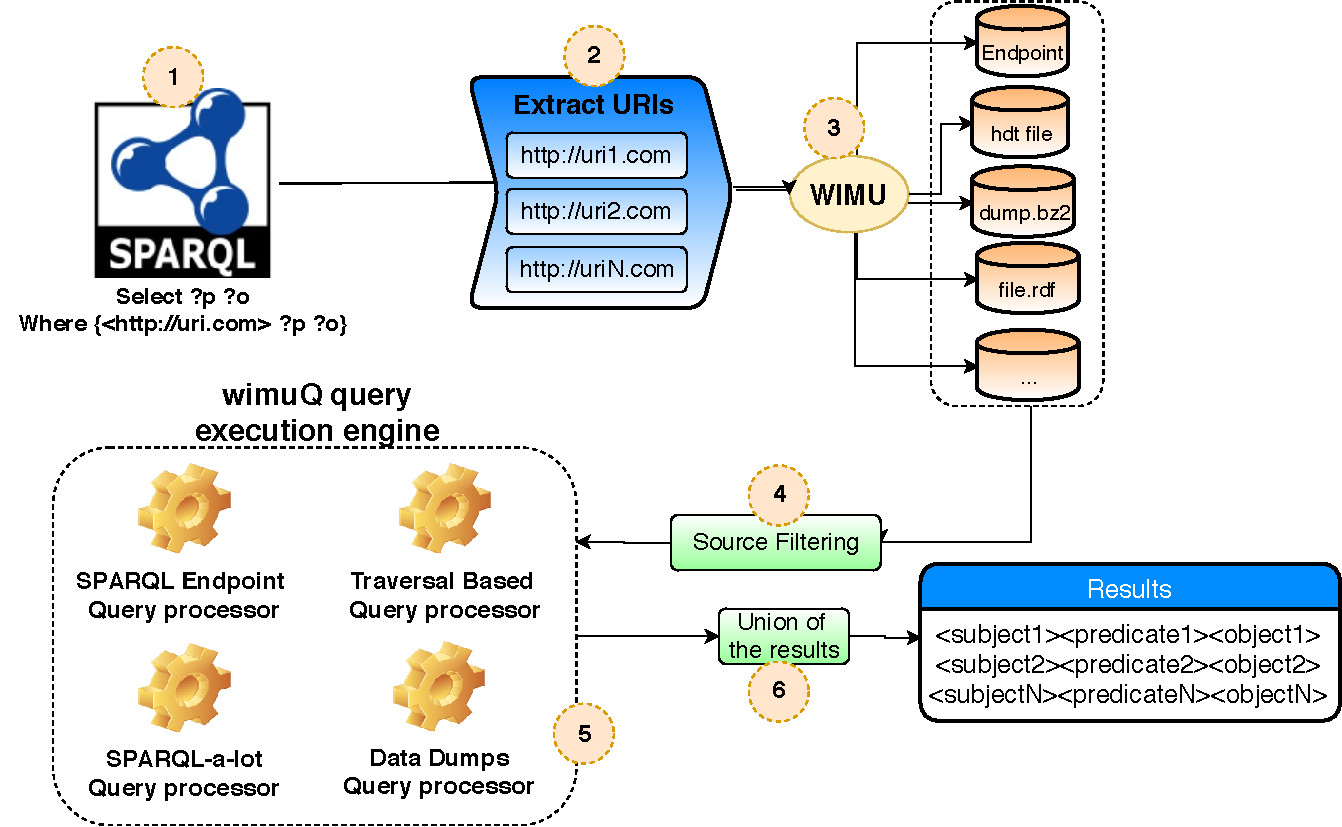
\includegraphics[width=\linewidth]{img/wimuT3.pdf}
	%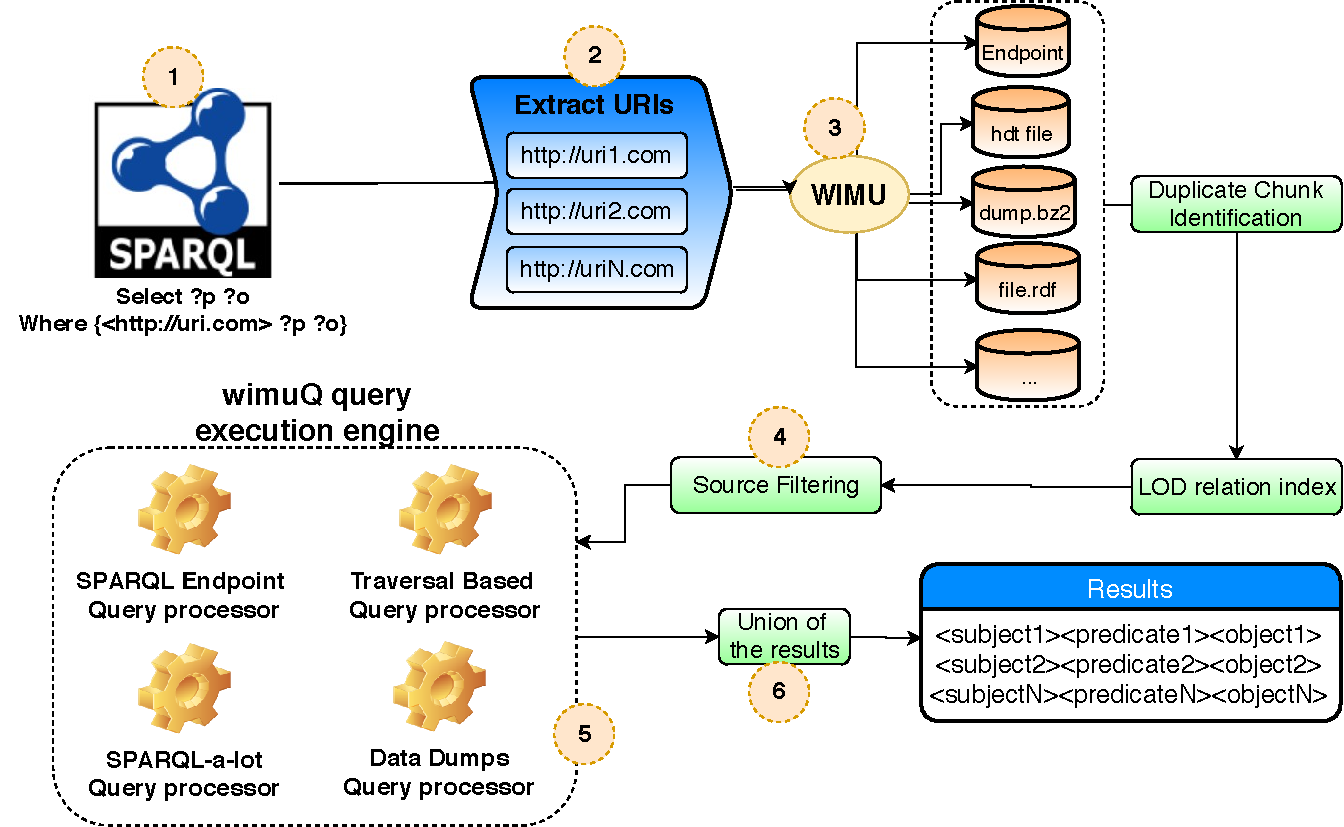
\includegraphics[width=\linewidth]{img/wimuqArq.pdf}
	\caption{WimuQ's query processing workflow.}
	\label{fig:approach}
\end{figure}

Now we go into the details of these steps, explaining the different components. 

\subsection{WimuQ source selection}
One of the important optimization steps in federated SPARQL query processing is the \emph{source selection} \cite{costfed2017,hibiscus2014}. The goal of the source selection is to identify the potentially relevant datasets (also called sources) to the given query. We make use of the WIMU service \cite{valdestilhas2018my} to select the potentially relevant sources. The WIMU service\footnote{WIMU URIs lookup service is available from: \url{http://wimu.aksw.org/}} provides URIs lookup facility and identify those datasets which contain the given URI. Currently, this service processed more than 58 billion unique triples and indexed 4.2 billion URIs from more than 660k RDF datasets obtained from the most used Linked Data hubs including LODStats~\cite{auer2012lodstats} and LOD Laundromat~\cite{beek2014lod}. The identified WIMU datasets can be of four types: (1) SPARQL endpoint, (2) HDT file, (3) dataset with dereferenceable URIs, (4) data dump with non-dereferenceable URIs. 
The service is both available from a web interface as well as can be queried from a client application using the standard HTTP protocol. 

The WimuQ source selection algorithm is given in Algorithm \ref{alg:iss1} which takes a SPARQL query $Q$ as input. We provide the set of extracted URIs (from step 2) $U$ to the WIMU service and retrieve the relevant datasets $D$ pertaining to the given URIs (Lines 1-4 of Algorithm \ref{alg:iss1}). Now for each relevant dataset $d$ $\in$ $D$, if the $d$ is a SPARQL endpoint, we extract the individual triple patterns $t$ of the query and perform a SPARQL ASK of $t$ in dataset $d$ (Lines 5-8 of Algorithm \ref{alg:iss1}). We add the dataset $d$ into the set of relevant SPARQL endpoints $E$, if the SPARQL ASK query returns true (Lines 9-13 of Algorithm \ref{alg:iss1}). We directly add $d$ into sets $H$ and $T$ if $d$ is an HDT file or if the $d$ is a SPARQL endpoint or dataset with dereferenceable URIs, respectively (Lines 14-19 of Algorithm \ref{alg:iss1}). Finally, if $d$ is dataset with non-dereferenceable URIs, we apply the RDFSlice \cite{marx2017torpedo} technique to only get the relevant RDF slice of the dataset. The RDF slice is then considered as a relevant dataset (Lines 20-23 of Algorithm \ref{alg:iss1}). The purpose of only adding the relevant slice of the complete dataset is to reduce the processing overhead, explained in the next section. 

\begin{algorithm} [htb] 
	\caption{The WimuQ source selection}
	\label{alg:iss1}
    %\begin{multicols}{2}
    	\textbf{Input}: $\mathbf{Q}$ \Comment{The SPARQL query} \\
    	\textbf{Output}: $\mathbf{E}, \mathbf{H}, \mathbf{T}, \mathbf{N}$  \Comment{Hash sets of relevant sources of SPARQL endpoints, HDT files, dataset with dereferenceable URIs, datadump with non-dereferenceable URIs, respectively  }
    	\begin{algorithmic}[1]
    	%	\Procedure{WimuQ($\mathbf{Q}$)}{}
    		%\State{$\mathbf{R}=\{\}$}
    		%\State{nU = 0}
    		\State{$\mathbf{U} = extractURIs(\mathbf{Q})$}  \Comment{Extract the URIs from the SPARQL query}
    		\ForAll{$\mathbf{u} \in \mathbf{U}$}
    		    \State{$\mathbf{D} = \mathbf{D} \cup wimuLookup(\mathbf{u})$} \Comment{Datasets from the WIMU}
    		   \EndFor
    		    \ForAll{$d \in \mathbf{D}$} \Comment{For each dataset} 
      	        \If{d is SPARQL endpoint}
    		        \ForAll{$t \in \mathbf{Q}$} \Comment{For each Triple pattern in query}
    		          	\State{ b = $ASK$(t,d)} \Comment{SPARQL ASK of t in d}
    		         \If{b = true}
    		            	\State{ $\mathbf{E}$.add(d) }
    		          \EndIf  		            
    		        \EndFor
     		    \EndIf
     		     \If{d is HDT file}
     		     	\State{ $\mathbf{H}$.add(d) }
     		     	\EndIf 
     		     	 \If{d is dataset with dereferenceable URIs}
     		     	\State{ $\mathbf{T}$.add(d) }
     		     	\EndIf 
     		     		 \If{d is datadump with non-dereferenceable URIs}
     		     	\State{ $\mathbf{N}$.add($RDFSlice$(d)) } \Comment{only add the relevant slice}
     		     	\EndIf
     		    \EndFor
     		  %  \State{eliminateDuplicates($\mathbf{H}$) }
     		  %  \EndFor
     		\State{return $\mathbf{E}, \mathbf{H}, \mathbf{T}, \mathbf{N}$} \Comment{ final relevant sources set}
    	%	\EndProcedure
    	\end{algorithmic}
	%\end{multicols}
\end{algorithm}

%%%%%%%%%%%%%%%%
\begin{comment}

\subsection{Identifying duplicates}
\label{sec:duplicates}
The function eliminateDuplicates(), identify and eliminate duplicated HDT files by comparing the property occurrences of each dataset and the header metadata.

We formalize the problem of Clustering datasets identifying duplicates and chunks as follows:

We consider a set of $\mathbf{K}$ data sources $\mathbf{S_1}, . . . , \mathbf{S_k}$ containing property occurrences $\mathbf{O_1}, . . . , \mathbf{O_m}$. Each of property $\mathbf{P}$ is referenced by an \texttt{URI}, e.g., dbo:City\footnote{dbo:City states for the URI \url{http://dbpedia.org/ontology/City}}. Each $\mathbf{S}$ contains a header $\mathbf{H}$, with meta-data about the data in $\mathbf{S}$, such that $\mathbf{H} \subset \mathbf{S}$.

The goal is to create clusters of datasets $\mathbf{C}$ in two groups of elements from $\mathbf{K}$, in which are duplicates $\mathbf{D}$ and chunks $\mathbf{E}$, such that $\mathbf{D} \subset \mathbf{K} : \mathbf{E} \subset \mathbf{K} : \mathbf{K} \subset \mathbf{C}$.

We assume that all datasets are not empty and are RDF compatible with the HDT format.

Firstly we create a dense matrix of property occurrence and dataset. Then it was observed a standard in the dense matrix, that for some datasets the occurrence of the properties was exactly the same. Then, we identify that we can put together those datasets to observe more characteristics.
At the next step, we have a sub-collection of our initial collection of datasets and looking into the header metadata of those files\footnote{In this step we take a small sample and evaluate manually to validate.} we observe that for some files the meta-data is different. Then we have another sub-collection of files with different headers,  where we realize that the files are chunks, also know as small parts of a bigger dataset.

Thus we can have two phases for identify dataset chunks and duplicates (1) Put together datasets that present the same occurrence of properties. (2) Automatically evaluating the content of the header metadata, separating the files with different header. Thus, we have two groups of files, in which, files with different header are chunks and the rest of selected files are duplicates\cref{note1}.

% \footnote{More details are available in the extended version of this paper \url{http://139.18.13.76:8082/KCAP_extended.pdf} and also directly at the implementation on \url{https://github.com/firmao/wimuT} and the specific implementation java class for this task: \url{https://github.com/firmao/wimuT/blob/master/src/org/wimu/datasetselection/parallelv1/ClusterKmeans.java}}.
%(2) Read the header metadata and separate files with a different header. The files with different header are chunks and the rest are duplicates

\subsection{The incremental LOD Dataset relation index}
\label{sec:index}
Persons will always describe the knowledge in a different way, due to the individuality of the being, different point of view, time and space, in which we assume as a natural phenomenon. We observe that the LOD datasets are following this standard and we are also aware of the state of the art from Ontology/Schema/Instance Matching from Linked Data from papers on venues such as VLDB, OEAI, ISWC, ESWC, among others.

In the LOD cloud, there are several similar datasets, but there is no place that store or provide such kind of information about how similar are the datasets, in our case, which properties the datasets share. The aim of this index is to store the relation among them in order to see how similar they are based on their properties\footnote{In this case properties makes also reference to predicates}.
Here we provide an index of the relation among properties of the LOD datasets.

The index\cref{guiweb} provides the following information based on three types of input:
(1) \textbf{Dataset}, in which provides a list of datasets, number of exact matched properties and number of similar\footnote{With the Jaro–Winkler similarity threshold greater than 0.9.} properties. (2) \textbf{Set of properties (URIs) separeted by comma}, which will result in a \textbf{Json} file containing the property and the list of datasets where this property were found by exact match and a table containing the matches by similarity with the following fields: \textbf{Property Source}: Representing the property found on the dataset source, \textbf{Property Target}: Representing the property found on the dataset target, \textbf{Dataset Source}: The name of the dataset source, \textbf{Dataset Target}: The name of the dataset target. (3) \textbf{SPARQL query}, in which the set of properties will be extracted from the SPARQL query and performs the same operation as \textbf{Set of properties (URIs) separeted by comma}.
% \begin{description}
%     \item \textbf{Dataset}: The index will provide a list of datasets, number of exact matched\footnote{Exact Match where the URI is exact the same following the principle of uniqueness of the URI} properties and number of similar\footnote{Similarity match occurs when the similarity of the URI is greater than 0.9 if less we perform Instance matching.} properties.
%     \item \textbf{Set of properties (URIs) separeted by comma}: 
%     \begin{itemize}
%         \item Json file containing the property and the list of datasets where this property were found by exact match.
%         \item A table containing the matches by similarity with the following fields:
%         \begin{description}
%             \item \textbf{Property Source}: Representing the property found on the dataset source.
%             \item \textbf{Property Target}: Representing the property found on the dataset target.
%             \item \textbf{Dataset Source}: The name of the dataset source.
%             \item \textbf{Dataset Target}: The name of the dataset target.
%         \end{description}
%     \end{itemize}
%     \item \textbf{SPARQL query}: This type of input extracts the set of properties from the SPARQL query and performs the same operation as \textbf{Set of properties (URIs) separeted by comma}.
% \end{description}

The index is also incremental, allowing to add more datasets to be processed once a month\footnote{Once a month due to the the time to generate that with our hardware takes at least 88 hours}. Our online prototype is available online\footnote{\label{guiweb}You can check our online prototype for proof of concept only about this LOD Dataset relation index at \url{http://139.18.13.76:8082/DatasetMatchingWeb/}.}

The current version of the index prototype has information about 539 SPARQL endpoints from LOD cloud\cref{endpoints} and 915 HDT files from LOD Laundromat\footnote{http://lodlaundromat.org/}. We perform more than 1,800,000 comparisons in 88 hours.

Now we give an example of a use of the index as following: Given a SPARQL query that works on CKAN SPARQL endpoint \url{https://linked.opendata.cz/sparql}:
\begin{verbatim}
Select * where { ?s ?p ?o.
Filter(?s=<http://purl.org/dc/terms/date> || 
?s=<http://crime.rkbexplorer.com/id/location> || 
?s=<http://purl.org/dc/terms/subject>
)}
\end{verbatim}
When we submit the SPARQL query to the index web interface\cref{guiweb} we can observe that the properties \url{http://purl.org/dc/terms/date}, \url{http://crime.rkbexplorer.com/id/location} and \url{http://purl.org/dc/terms/subject} are found in other datasets, which means, besides the SPARQL endpoint \url{https://linked.opendata.cz/sparql}, the query can be executed in at least 5 more datasets, for example, \url{https://eu.dbpedia.org/sparql}, likely complementing the results. Another important observation was related to ontology alignment of SPARQL endpoints from the same type\footnote{we refer to SPARQL endpoints sharing a base ontology, in case DBpedia endpoints}, for example, the query works at \url{https://eu.dbpedia.org/sparql} but not at \url{http://dbpedia.org/sparql}\footnote{\label{note1}More details are available in the extended version of this paper at \url{http://139.18.13.76:8082/KCAP_extended.pdf}}.
\end{comment}
% Thanks to the index we are able to know that we can also execute the query at \url{https://eu.dbpedia.org/sparql} but not at \url{http://dbpedia.org/sparql}, and we can execute at least in more 5 datasets also complementing the results. More details are available in the extended version of this paper\footnote{\label{note1}The extended version of this paper is available at \url{http://139.18.13.76:8082/KCAP_extended.pdf}}.

\subsection{WimuQ query execution}
We make use of the four -- SPARQL endpoint, Link Traversal-based, SPARQL-a-alot, Data dumps -- query processor to execute federated queries over the aforementioned four types of WIMU datasets. The relevant data sources for each of these query processors are returned by the WimuQ source selection discussed in previous section. 

In WimuQ, we used FedX \cite{fedx2011} query processor for SPARQL endpoints query federation and SQUIN for traversal-based query federation. The reason for choosing FedX for SPARQL endpoints federation and SQUIN for traversal-based federation is due the fact that they do not require any pre-computation of dataset statistics and hence are able to retrieve up-to-date results. Thus both are able to run federated queries with zero initial knowledge. In addition, both produce reasonably query runtime performances comparing to state-of-the-art approaches \cite{saleem2015fine,saleem2018costfed,hartig2013squin}.

The list of required endpoints URLs for FedX are returned from the previously discussed source selection Algorithm (ref. $\mathbf{E}$ of Algorithm \ref{alg:iss1}). The potentially relevant dereferenceable URIs data sources (ref. $\mathbf{T}$ of Algorithm \ref{alg:iss1}) are already identified by the WimuQ sources selection algorithm. Thus, we reduced the search space by only considering the dereferenceable URIs data sources. 
 
As mentioned before, FedX can only works with public SPARQL endpoints. SQUIN needs dereferenceable URIs. Both of these engines are unable to execute SPARQL queries over non-dereferenceable URIs datadumps: SPARQL endpoint federation approaches cannot execute queries over such datadumps as they are not exposed as SPARQL endpoints, link traversal-based approaches fail to retrieve results as the URIs are non-dereferenceable. We need to download the dumps first, load it locally, and run some query processing API (e.g., JENA or Sesame) on the loaded datasets. However, we can not simply download the complete dumps and process it locally due to their large amount of data. To solve this problem, we make use of the Wimu index to only select those data dumps which are potentially capable to execute the given query. These datadumps are further sliced by using the RDFSlice technique, to only select the required chunks of the datadumps which will provide results to the given SPARQL query. The identified chunks are finally loaded in a local Apache Jena model. The model is then use to execute federated queries. 

Finally, we propose a query processor named \emph{SPARQL-a-lot} to execute federated SPARQL queries over HDT files. The SPARQL-a-lot is a CBD-based\footnote{\label{cbd}\url{https://www.w3.org/Submission/CBD/}} query execution described in Algorithm \ref{alg:sparqlAlot}. The algorithm takes a SPARQL query $Q$ as input and return the resultset $O$ of the query execution over HDT file. First, the algorithm extracts all of the BGPs from Q (Line 2 of Algorithm \ref{alg:sparqlAlot}). The next step is to extract the subjects, predicates, and objects of all the triple patterns used in $Q$ (Line 3 of Algorithm \ref{alg:sparqlAlot}). The CBDs are then generated from extracted subjects, predicates, and objects (Line 4 of Algorithm \ref{alg:sparqlAlot}). The extracted CBDs constitute an RDF dataset of set of triples $T$ which are then loaded into a local Jena model (Line 5 of Algorithm \ref{alg:sparqlAlot}). The query $Q$ is then finally executed over the Jena model and results are returned (Lines 6-7 of Algorithm \ref{alg:sparqlAlot}). The duplicated results from different query processing engines is removed after collecting the final results. 


\begin{algorithm} [htb] 
	\caption{Query execution on LOD-a-lot}
	\label{alg:sparqlAlot}
    %\begin{multicols}{2}
    	\textbf{Input}: $\mathbf{Q}$ \Comment{The SPARQL query} \\
    	\textbf{Output}: $\mathbf{O}$ \Comment{The results of the query}
    	\begin{algorithmic}[1]    		
            \Procedure{sparql-a-lot($\mathbf{Q}$)}{}
        		\State{$\mathbf{BGP} = extractBGP(\mathbf{Q})$}  \Comment{Extract the BGP from the SPARQL query}
        		\State{$\mathbf{Tbgp}$ = extractSPO($\mathbf{BGPs}$)} 
        		\State{$\mathbf{T}$ = executeAPILOD-a-LOT($\mathbf{Tbgp}$)} \Comment{Generating CBDs from $s,p,o$}
        		\State{createTDBJena($\mathbf{T}$)}
        		\State{$\mathbf{O}$ = execSPARQLTDBJena($\mathbf{Q}$)}
        		\State{return $\mathbf{O}$}
    		\EndProcedure
    	\end{algorithmic}
	%\end{multicols}
\end{algorithm}

The results generated by each of WimuQ's processors are finally integrated and sent back to the user. 

 \subsection{Practical example}
 Given the following SPARQL query (LD1 from FEDBench\cite{fedbench2011}):

 \begin{verbatim}
 PREFIX rdfs: <http://www.w3.org/2000/01/rdf-schema#>
 SELECT * WHERE { ?paper 
 <http://data.semanticweb.org/ns/swc/ontology#isPartOf> 
 <http://data.semanticweb.org/conference/iswc/2008/
 poster_demo_proceedings> .
 ?paper <http://swrc.ontoware.org/ontology#author> ?p .
 ?p rdfs:label ?n .
 }
 \end{verbatim}

 
% In which the query asks for all information\footnote{All information refers to all triples.} about author names that have papers at poster-demo proceedings from ISWC 2008.

% We can identify six possible different types of problem: (1) the SPARQL endpoint is not available anymore, (2) there are no dump-files, (3) the URIs are not dereferenceable anymore, (4) the dataset is incomplete, (5) the user needs to query more than one dataset for the same query and (6) the user does not know where to execute the query.

% Several approaches have been proposed to deal with the problem of executing a SPARQL query on heterogeneous sources, but the user should know the dataset in advance, none of them propose a solution to identify the best collection of datasets able to execute a query.

% Also, there is no approach in which is able to execute a query in a very large collection of datasets, (i.e., query datasets from LOD cloud, LOD Laundromat and LODStats), due to the still open problem of ontology/schema matching on very large heterogeneous collection of datasets\footnote{very large, we refer to more than 600,000 datasets}.

% To deal with the problem we also studied the state of the art of ontology/schema matching, selecting the most related papers \cite{stoilos2018novel,skjaeveland2018practical,oliveira2018improving}.

% Some of these works are competitive (i.e., serve identical needs), while others are complementary, as their combination leads to better performance. However, there is no systematic study on how these methods relate to each other to serve a common purpose.

With WimuQ we were able to identify 4 HDT datasets available from 
\url{https://tinyurl.com/WimuQexData}. All of these datasets are
from LOD Laundromat repository~\cite{beek2014lod} containing information about the conference ISWC2008~\cite{sheth2008semantic}, under the domain \url{http://data.semanticweb.org}, originally from SW Dog Food dataset\footnote{\url{https://old.datahub.io/dataset/semantic-web-dog-food}}. Thus, \emph{SPARQL-a-lot} is the only query processing engine (because of the selected datasets are HDTs) which is considered for executing the given SPARQL queries. The final results of the query execution is available from \url{https://tinyurl.com/WimuQExample}. 



\section{Evaluation}
\label{sec:eval}
%To verify our hypothesis, in this section we evaluate if we can access the datasets from URIs not dereferenceable anymore, we can improve the source selection and have better coverage of the results from a SPARQL query.
In this section, we present the evaluation setup and the corresponding results that validate our hypothesis that we can improve the resultset retrieval if we automatically identify potentially relevant sources from heterogeneous RDF data even if the URIs are not dereferenceable anymore. The goal of this evaluation is to show that by combining different SPARQL query processing approaches, we are able to retrieve more complete results as compared to the results retrieved by the individual approaches. 
\subsection{Experimental setup}

\subsubsection{Benchmarks used:} Since WimuQ aims to execute SPARQL queries over real-world RDF datasets, we chose three -- FedBench \cite{fedbench2011}, LargeRDFBench \cite{largerdfbench2017}, Feasible \cite{feasible2015} -- real-world RDF datasets benchmarks in our evaluation: 
\begin{itemize}
  
\item \textbf{FedBench} is federated SPARQL querying benchmarks. It comprises of a total of 25 queries and 9 real-world interconnected datasets. FedBench queries are further divided into three main categories: (1) 7 queries from Life Sciences (LS) domain, (2) 7 queries from Cross Domain (CD), and (3) 11 queries named Linked Data (LD) for link traversal-based approaches. The detailed statistics of the benchmark's datasets and queries are given in FedBench\cite{fedbench2011}.

\item  \textbf{LargeRDFBench} is also a federated SPARQL querying benchmark. It comprises a total of 40 queries and 13 real-world interconnected datasets. FedBench queries are further divided into four main categories: (1) 14 \emph{Simple} queries, (2) 10 \emph{Complex} queries, (3)  8 \emph{Large Data} queries, and (4) 8 \emph{Complex+High Data Sources} queries. The detailed statistics of the benchmark's datasets and queries are given in \cite{largerdfbench2017}. 

\item  \textbf{FEASIBLE} is a benchmark generation framework which generates customized benchmarks for the queries logs. In our evaluation, we chose exactly the same benchmarks used in \cite{feasible2015}: (1) 175 queries benchmark generated from DBpedia queries log and (2) 175 queries benchmark generated from Semantic Web Dog Food (SWDF) queries log. Further advanced statistics of the used datasets and queries can be found in \cite{feasible2015}. 
\end{itemize}
To the best of our knowledge, these are the state-of-the-art from the real-data SPARQL benchmarks. All of the 415 queries used in our evaluation is publicly available\footnote{Queries available from \url{https://github.com/firmao/wimuT/blob/master/queriesLocation.txt}}. 

\subsubsection{Hardware:} All the experiments were done on a modest machine with 200 GB of Hard Disk, 8 GB of RAM and a 2.70GHz single core processor. Each of the queries was run 5 times and the average of the results are presented.  

\subsubsection{SPARQL endpoints:} As previously stated, the query federation over multiple SPARQL endpoints approaches requires the set of endpoint URLs to be provided as input to the federation engine. We chose a total of 539 active SPARQL endpoints available from LOD cloud\footnote{List of SPARQL endpoints: \url{https://lod-cloud.net/lod-data.json}}. We filtered the endpoints URLs\footnote{\label{endpoints}Endpoints URLs with size: \url{https://goo.gl/H2t5ko}} and the total number of triples hosted by each of these endpoints. 

\subsubsection{Metrics:} Since WimuQ aims to retrieve more complete results within the reasonable amount of time, we choose two metrics: (1) coverage in terms of the number of results retrieved from the query executions and (2) the time taken to execute the benchmark queries. 

\subsubsection{Approaches:} As mentioned in Section \ref{sec:related}, different federation engines available to federate SPARQL queries over endpoints and traversal-based federation. We chose FedX \cite{fedx2011} for SPARQL endpoint federation and SQUIN \cite{hartig2013squin} for traversal-based query federation. The reason for choosing these two engines is due the fact they do not require any pre-computation of dataset statistics and hence able to retrieve up-to-date results and able to run federated queries with zero initial knowledge. In addition, both these engines perform reasonably well in terms of query runtime performances w.r.t state-of-the-art approaches \cite{saleem2015fine,saleem2018costfed,hartig2013squin}. For the sake of completeness, we also compared WimuQ with SPARQL-a-lot and WimuDumps.  

%In total, we processed more than 5 Terabytes of information from datasets retrieved using WIMU. None of ours experiment SPARQL query setups occupied more than 200 GB in disk. The source-code to reproduce the experiments is available online\footnote{\url{https://github.com/firmao/wimuT}}.
%In case, the machine do not need to have more than 200 GB, because we start discarding the datasets when reach the limit of 200 GB according to the use
\subsection{Results}
\textbf{Coverage of the results}: The main purpose of WimuQ is to devise a federation engine which is able to retrieve more complete results for the given SPARQL queries. %One of the most important results is the coverage of the results achieved by using each selected methods to compose the WimuQ. 
\Cref{fig:numberRes1} shows a comparison of the selected approaches in terms of the average of the number of results retrieved for the different queries categories of the selected benchmarks. The complete results for individual queries can be found on our aforementioned project website. By using different query processing engines, our approach is able to retrieve more results as compared to the results retrieved by only using SPARQL endpoints federation engine (i.e, FedX) link traversal engine (i.e., SQUIN), data dumps, or  HDT files. In our evaluation, the average resultset size of WimuQ is 8481 across the three benchmarks. Out of these, WimuQ collects about 91\% of the results from wimuDumps (avg. resultset size 7651), 7\% from SPARQL endpoints (avg. resultset size 556), and 1\% from SPARQL-a-lot (avg. resultset size 74). 

\begin{figure}[htb]
    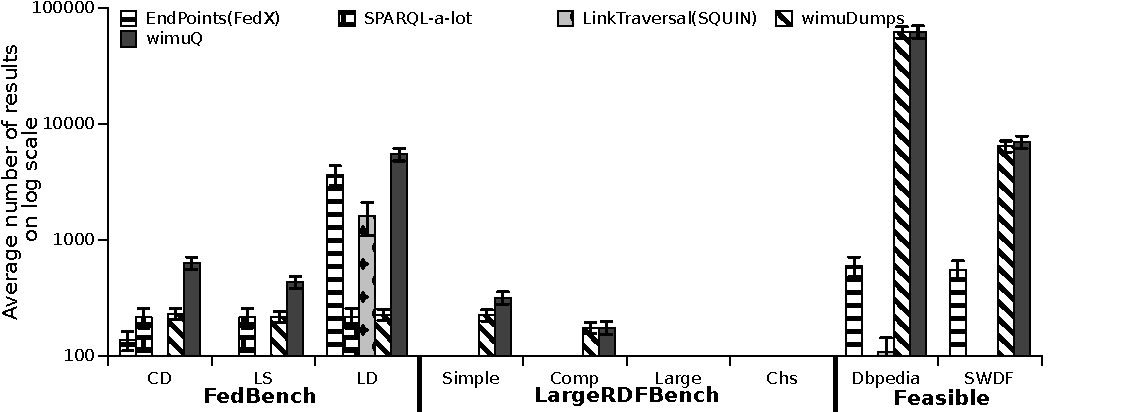
\includegraphics[width=\linewidth]{img/numberRes1.pdf}
	\caption{Average number of results retrieved by the selected approaches across different queries categories of the selected benchmarks.}
	\label{fig:numberRes1}
\end{figure}

For FedBench, the WimuQ avg. resultset size is 2,253. Out of these results, about 55\% are collected from SPARQL endpoints by using FedX query processing engines (avg. resultset size 1,262). The LinkTraversal (SQUIN) contributed about 25\% of the total results (avg. resultset size 549), wimuDumps contributed about 10\% of the total results (avg. resultset size 226), and SPARQL-a-lot also contributed about 10\% of the results (avg. resultset size 215). 

For LargeRDFBench, the WimuQ avg. resultset size 123. Out of these results, about 81\% are collected from wimuDumps (avg. resultset size 100). The SPARQL endpoints contributed about 14\% of the results (avg. resultset size 17). The LinkTraversal(SQUIN) contributed 6\% of the total results (avg. resultset size 6), and SPARQL-a-lot did not provide results (avg. resultset size 0). 

For FEASIBLE, the WimuQ avg. resultset size 34,537. Out of these results, about 98\% are collected from wimuDumps (avg. resultset size 33,893). The SPARQL endpoints contributed about 1.6\% (avg. resultset size 577). The LinkTraversal(SQUIN) approach contributed only about 0.15\% (avg. resultset size 54). Finally, SPARQL-a-lot query processing engine only retrieved about 0.03\% results (avg. resultset size 11). 

In summary, WimuQ is able to retrieve at least one resultset for 76\% of the overall 415 queries. The results clearly shows that by combining different query processing engines into a single SPARQL query execution framework lead towards more complete resultset retrieval. 
An important observation is that the selected approaches are mostly not able to retrieve results for the Large Data and Complex+High (Ch) queries categories of LargeRDFBench. The reason is getting zero results for the Large Data queries is that these queries retrieve results from the LinkedTCGA \cite{tcga2013} datasets which were not publicly available via SPARQL endpoints, were not indexed by WIMU, also were not reachable via link traversals. While Ch queries often require higher number of distributed datasets in order to compute the final resultset of the queries. Thus, the approaches were able to find all of the relevant datasets, required to compute the final resultset of the queries. The average number of datasets\footnote{Here we also point the number of datasets discovered} queries by WimuQ for the selected benchmarks queries categories in given in Figure \ref{fig:numberDatasets1}. We can clearly see the highest number of datasets are selected for Ch queries of LargeRDFBench. 

\begin{figure}[htb]
\centering
    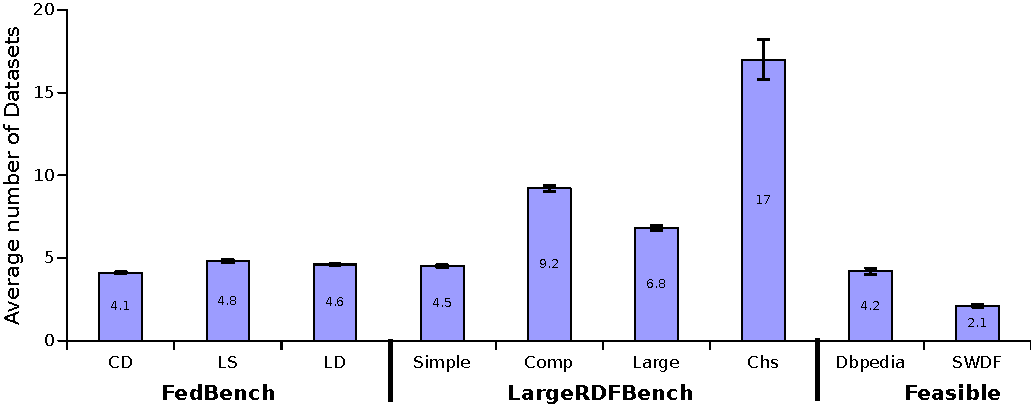
\includegraphics[width=\linewidth]{img/numberDatasets1.pdf}
	\caption{Average number of datasets discovered and queried by WimuQ across different queries categories of the selected benchmarks.}
	\label{fig:numberDatasets1}
\end{figure}

\textbf{Query runtime performances}: 
\Cref{fig:runtime1} shows a comparison of the selected query processing engines in terms of the average query run times for the different queries categories of the selected benchmarks. The average query runtime of WimuQ is 17 minutes across the three benchmarks. The average query execution to collect results from wimuDumps is about 2 minutes, which in turn is followed by query execution over SPARQL endpoints (avg. query runtime 13 minutes), SPARQL-a-lot (avg. query runtime 58 seconds) and LinkTraversal (SQUIN) (avg. query runtime 36 seconds). Interestingly, WimuQ collects about 91\% of the results from wimuDumps yet its average execution time is smaller than query execution over SPARQL endpoints which provide only 7\%  of the total results. One possible reason for this could be that in SPARQL endpoint federation, the query processing task split among multiple selected SPARQL endpoints and hence network and the number of intermediate results play an important role in the quer runtime performances. 

For FedBench, the WimuQ average query runtime 20 minutes. Out of this, the average avg. query runtime over SPARQL endpoints is 16 minutes, followed by wimuDumps (avg. query runtime 2 minutes), LinkTraversal (SQUIN) (avg. query runtime 49 seconds), and SPARQL-a-lot (avg. query runtime 46 seconds), respectively. For LargeRDFBench, the average query execution of WimuQ is 11 minutes. Out of this query execution over SPARQL endpoints took 8 minuts on average, followed by wimuDumps (avg. query runtime 2 minutes), SPARQL-a-lot (avg. query runtime 35 seconds), and LinkTraversal (SQUIN) (avg. query runtime 25 seconds), respectively. For FEASIBLE, the WimuQ takes on average of 24 minutes per query execution. Out of this, the query federation over SPARQL endpoints took about 18 minutes on average. Which is followed by wimuDumps (avg. query runtime 3 minutes), SPARQL-a-lot (avg. query runtime 1), and LinkTraversal (SQUIN) (avg. query runtime 36 seconds), respectively.

As an overall query runtime evaluation, we can clearly see there is a trade-off between the recall and query runtimes: the highest the recall the highest the query runtimes. Finding a balance between the recall and runtime would be an interesting research question to be considered in the future.  

\begin{figure}[htb]
    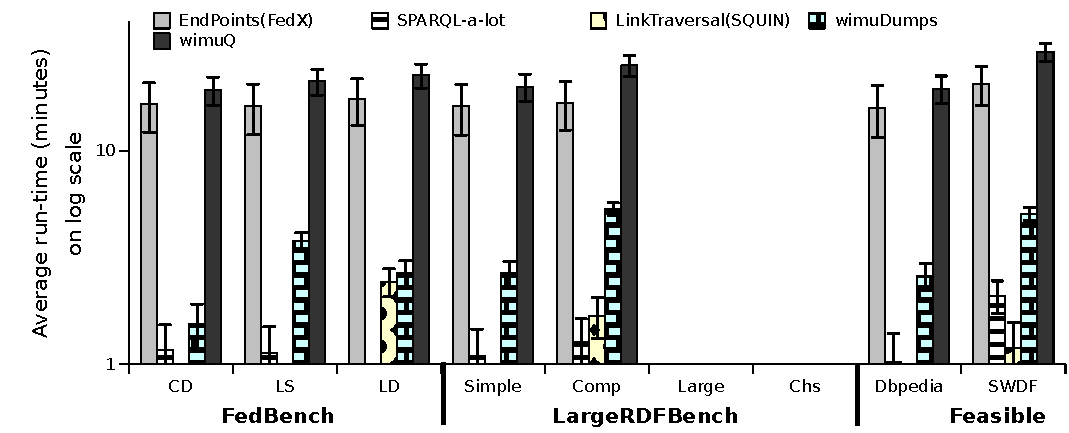
\includegraphics[width=\linewidth]{img/runtime1Min.pdf}
	\caption{Average query runtimes of the selected approaches across different queries categories of the selected benchmarks.}
	\label{fig:runtime1}
\end{figure}

The results of our evaluation lead us to validate our hypothesis that we can improve the resultset retrieval if we identify potentially relevant sources from heterogeneous RDF data.

% \section{Conclusions and Future Work}
% \label{sec:conc}
% \textit{}
